\documentclass[12pt]{extarticle}
\usepackage[utf8]{inputenc}
\usepackage{cite}
\usepackage{float}
\usepackage{hyperref}
\usepackage{graphicx}
\graphicspath{./}

\title{Path Planning in Unknown Environment with Obstacles Using RRT*-SMART}
\author{
	Sagar Ojha \\
	\texttt{as03050@umd.edu}
	\and
	Obaid Ur Rahman\\
	\texttt{obdurhmn@umd.edu}}
\date{\today}

\begin{document}
\maketitle
\newpage
%---------------------------------------------------------------------------------------------------
%---------------------------------------------------------------------------------------------------
\section{Introduction}
\hspace{\parindent}For our final project, we propose to implement Rapidly Exploring Random Tree Star Smart (RRT*-Smart) algorithm in an obstacle-filled environment. It is a modified version of the Rapidly Exploring Random Tree Star (RRT*) algorithm and it has been shown to be effective in path planning problems. RRT*-Smart employs a novel approach that combines two new techniques in addition to RRT*, path optimization and intelligent sampling.

Path planning is a crucial task in robotics and automation, and several methods have been suggested to address this issue. One of the most popular methods for resolving path planning issues is the Rapidly Exploring Random Tree (RRT) algorithm, which LaValle and Kuffner \cite{La} initially presented in 1998. RRT is a probabilistic technique that builds a tree of viable robot configuration options. It is a widely used algorithm for path planning in robotics. The algorithm builds a tree of feasible paths in the configuration space of a robot from a randomly sampled nodes. The new nodes are added to the tree by selecting a nearby node and extending the tree towards a randomly sampled configuration. This process is repeated until a feasible path from the initial configuration to the goal configuration is found. The method has been extended and modified by a number of researchers to enhance the performance of RRT. One such modification is RRT-Connect method, which was put forth by Karaman and Frazzoli in 2000. This version constructs two trees from the beginning and goal configurations and links them to produce a path.

The produced pathways may not be optimal, nevertheless, because of the original RRT method. In 2010, Karaman and Frazzoli devised the RRT* method to overcome the optimality problem. In order to increase the number of optimum pathways, RRT* builds a more balanced tree and rewires the tree structure. The algorithm achieves convergence towards the best solution, assuring asymptotic optimality as well as probabilistic completeness. Yet, it has been demonstrated that it is time consuming and has a slow convergence rate especially when there are complicated obstacles.

As a result, RRT*-Smart was proposed to address limitations of RRT*. It was introduced by Jauwairia Nasir et al. in 2013 \cite{Jau}. The algorithm uses heuristic information to direct sampling toward the objective region. Thus, it accelerates the rate of convergence in order to arrive at an optimal or near-optimal solution considerably faster, thereby lowering execution time. The algorithm's innovative method takes use of two new approaches  in addition to RRT*, path optimization and intelligent sampling, which we will be implementing as our final project. 

In terms of computing efficiency and route quality, RRT*-Smart has been demonstrated to perform better than previous RRT-based algorithms.

%---------------------------------------------------------------------------------------------------
\section{Goal}
\hspace{\parindent}The goal of the project is the practical implementation of RRT*-Smart and a written technical report, and presentation. Below is the list of complete goals.

\begin{enumerate}
	\item Implementation of RRT*-Smart, a cutting-edge sampling based path-planning technique presented by Nasir J et al. \cite{Jau}, in simulation.
	\item A 6-8 page technical report in LaTex written in two column IEEE conference format describing introduction/motivation, a brief background and related work, methodology including high-level pseudo code and system details, tests/demos/experiments that were run, discussion, conclusions, and bibliography.
	\item In class presentation with 10-12 slides.
\end{enumerate}

The simulation will be performed using Gazebo and OpenCV. The primary goal will be the implementation of RRT*-Smart that is capable of precisely and efficiently guiding a robot in a given area with obstacles. The algorithm's performance will be assessed using a variety of measures, including path length, computing time, and obstacle avoidance.

%---------------------------------------------------------------------------------------------------
\section{Method}
\hspace{\parindent}The path planning method is sampling-based and it will be forward search using RRT*-Smart. The title of the paper that we will be implementing is ``RRT*-SMART: A Rapid Convergence Implementation of RRT*" by Nasir, J et al\cite{Jau}.

The algorithm is as shown in Figure\ref{algo}.
\begin{figure}[H]
	\centering
	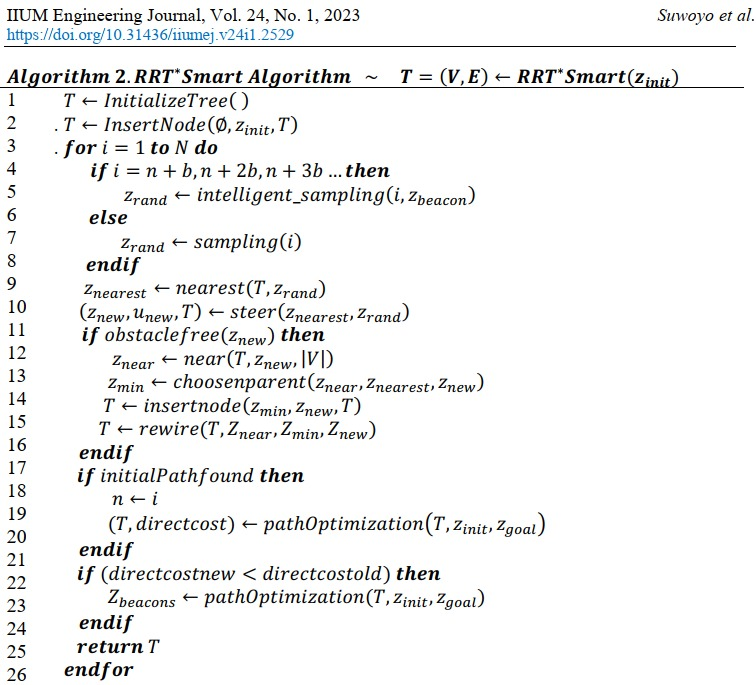
\includegraphics[scale = 0.5]{pseudocode}
	\caption{The algorithm for RRT*-Smart. \cite{Iram}}\label{algo}
\end{figure}

Below are the software packages and libraries in Python that we plan to use.
\begin{itemize}
	\item Gazebo
	\item ROS
	\item Rviz
	\item Numpy
	\item OpenCV
	\item Heapq
\end{itemize}

%---------------------------------------------------------------------------------------------------
\section{Timetable}

\begin{enumerate}
	\item Literature Review (5 days)
	\begin{itemize}
		\item Reading and analyzing papers (3 days)
		\item Understanding key concepts and algorithms (2 days)
	\end{itemize}
	
	\item Software setup and simulation environment (5 days)
	\begin{itemize}
		\item Installing software and packages (1 day)
		\item Setting up the simulation environment (4 days)
	\end{itemize}
	
	\item Implementation of RRT*-Smart (20 days)
	\begin{itemize}
		\item Implementing the algorithm (12 days)
		\item Testing in simulation (8 days)
	\end{itemize}

	\item Evaluation and optimization (5 days)
	\begin{itemize}
		\item Evaluating algorithm performance (2 days)
		\item Optimizing the algorithm (3 days)
	\end{itemize}

	\item Documentation and report writing (6 days)
	\begin{itemize}
		\item Writing the documentation (1 day)
		\item Writing the report (3 days)
		\item Preparing the presentation (2 days)
	\end{itemize}
\end{enumerate}
%---------------------------------------------------------------------------------------------------
\newpage
%---------------------------------------------------------------------------------------------------
\begin{thebibliography}{9}
	\bibitem{La}
	\href{http://lavalle.pl/papers/Lav98c.pdf}{LaVelle S, et al. ``Rapidly-Exploring Random Trees : A New Tool for Path Planning.”}

	\bibitem{Jau}
	\href{https://journals.sagepub.com/doi/10.5772/56718}{Nasir J, Islam F, Malik U, et al. ``RRT*-SMART: A Rapid Convergence Implementation of RRT*". International Journal of Advanced Robotic Systems. 2013;10(7). doi:10.5772/56718}
	
	\bibitem{Iram}
	\href{http://paper.ijcsns.org/07_book/201610/20161004.pdf}{Noreen I, et al. ``A Comparison of RRT, RRT* and RRT* -Smart Path Planning Algorithms". IJCSNS}
\end{thebibliography}

\end{document}